% This LaTeX was auto-generated from MATLAB code.
% To make changes, update the MATLAB code and export to LaTeX again.

\documentclass{article}

\usepackage[utf8]{inputenc}
\usepackage[T1]{fontenc}
\usepackage{lmodern}
\usepackage{graphicx}
\usepackage{color}
\usepackage{hyperref}
\usepackage{amsmath}
\usepackage{amsfonts}
\usepackage{epstopdf}
\usepackage[table]{xcolor}
\usepackage{matlab}

\sloppy
\epstopdfsetup{outdir=./}
\graphicspath{ {./topt_p2_antonio_fernandez_andres_herencia_images/} }

\matlabhastoc

\begin{document}

\label{T_B44F81CE}
\matlabtitle{\textbf{PRACTICE 2 - OPTIMIZATION TECHNIQUES}}

\begin{par}
\begin{flushleft}
\textbf{Andrés Herencia y Antonio Fernández}
\end{flushleft}
\end{par}

\begin{par}
\begin{flushleft}
\textbf{MUTECI 2023-2024}
\end{flushleft}
\end{par}

\matlabtableofcontents{Table of Contents}

\label{H_600AA6D1}
\matlabheading{Exercise 1}

\begin{par}
\begin{flushleft}
Given the data from the text file titled 'isomerizacion.txt,' determine the parameters that fit the model:
\end{flushleft}
\end{par}

\begin{par}
$$y=\frac{\theta_1 \theta_2 (x_2 -x_3 )/1.632}{1+\theta_2 x_1 +\theta_3 x_2 +\theta_4 x_3 }$$
\end{par}

\begin{par}
\begin{flushleft}
Request: 
\end{flushleft}
\end{par}

\begin{par}
\begin{flushleft}
a. Linearize the model and obtain an initial estimate. 
\end{flushleft}
\end{par}

\begin{par}
\begin{flushleft}
b. With the previous initial estimate, solve the non-linear regression problem by minimizing the squared error.
\end{flushleft}
\end{par}

\label{H_15EA53F7}
\matlabheadingtwo{Solution}

\begin{matlabcode}
clc
[x1,x2,x3,y]=textread('isomerizacion.txt','%f %f %f %f','headerlines',8);
\end{matlabcode}

\label{H_38C94BBB}
\matlabheadingthree{a) Linearize the model and obtain an initial estimate. }

\begin{par}
\begin{flushleft}
With $y^{\prime } =\frac{1}{y}(x_2 -x_3 )$ we can operate to achieve this expression:   $y^{\prime } =(x_2 -x_3 )\frac{1+\theta_2 x_1 +\theta_3 x_2 +\theta_4 x_3 }{\theta_1 \theta_2 (x_2 -x_3 )/1.632}=\frac{1.632}{\theta_1 \theta_2 }(1+\theta_2 x_1 +\theta_3 x_2 +\theta_4 x_3 )=\beta_0 +\beta_1 x_1 +\beta_2 x_2 +\beta_3 x_3$.
\end{flushleft}
\end{par}

\begin{par}
\begin{flushleft}
Where: $\theta_1 =\frac{1.632}{\beta_1 }$, $\theta_2 =\frac{\beta_1 }{\beta_0 }$, $\theta_3 =\frac{\beta_2 }{\beta_0 }$, $\theta_4 =\frac{\beta_3 }{\beta_0 }$.
\end{flushleft}
\end{par}

\begin{matlabcode}
X1 = [ones(length(x1),1),x1,x2,x3];
Y1 = [(x2-x3)./y];
beta = inv(X1.'*X1)*X1.'*Y1
\end{matlabcode}
\begin{matlaboutput}
beta = 4x1    
   -5.3459
    0.0396
    0.1798
   -0.3108

\end{matlaboutput}
\begin{matlabcode}
O(1)=1.632/beta(2);
O(2)=beta(2)/beta(1);
O(3)=beta(3)/beta(1);
O(4)=beta(4)/beta(1);
display(O)
\end{matlabcode}
\begin{matlaboutput}
O = 1x4    
   41.1949   -0.0074   -0.0336    0.0581

\end{matlaboutput}

\label{H_4A613B22}
\matlabheadingthree{b) With the previous initial estimate, solve the non-linear regression problem by minimizing the squared error.}

\begin{par}
\hfill \break
\end{par}

\begin{matlabcode}
f = @(x1,x2,x3,y,E) sum((y - (((x2 - x3)./1.632).*(E(1).*E(2)))./(1 + E(2).*x1 + E(3).*x2 + E(4).*x3)).^2);
myfunc = @(E) f(x1,x2,x3,y,E);
[beta_opt, fval, exitflag, output] = fminsearch(myfunc,O)
\end{matlabcode}
\begin{matlaboutput}
beta_opt = 1x4    
    4.7969   -0.0071   -0.0059    0.0200

fval = 210.4719
exitflag = 1
output = 
    iterations: 241
     funcCount: 409
     algorithm: 'Nelder-Mead simplex direct search'
       message: 'Optimization terminated:↵ the current x satisfies the termination criteria using OPTIONS.TolX of 1.000000e-04 ↵ and F(X) satisfies the convergence criteria using OPTIONS.TolFun of 1.000000e-04 ↵'

\end{matlaboutput}

\begin{par}
\begin{flushleft}
We can check that since the problem is non-linear, is very sensitive to the initial conditions and the optimization method, so, we can not interpretate the solution with ease.
\end{flushleft}
\end{par}

\begin{matlabcode}
[beta_opt2, fval2, exitflag2, output2] = fminunc(myfunc,O)
\end{matlabcode}
\begin{matlaboutput}
Local minimum found.

Optimization completed because the size of the gradient is less than
the value of the optimality tolerance.

<stopping criteria details>
beta_opt2 = 1x4    
   40.1275   -9.7344  -11.7309   -6.8991

fval2 = 16.1631
exitflag2 = 1
output2 = 
       iterations: 66
        funcCount: 350
         stepsize: 1.5932
     lssteplength: 1
    firstorderopt: 0.5222
        algorithm: 'quasi-newton'
          message: 'Local minimum found.↵↵Optimization completed because the size of the gradient is less than↵the value of the optimality tolerance.↵↵<stopping criteria details>↵↵Optimization completed: The first-order optimality measure, 6.264512e-07, is less ↵than options.OptimalityTolerance = 1.000000e-06.'

\end{matlaboutput}

\begin{par}
\begin{flushleft}
If we want to minimize the quadratic sum of errors, we have to use this method, because the fval parameter is the lowest.
\end{flushleft}
\end{par}

\begin{matlabcode}
[beta_opt3, fval3, exitflag3, output3] = fminsearch(myfunc,[0,0,0,0])
\end{matlabcode}
\begin{matlaboutput}
beta_opt3 = 1x4    
    0.0056    0.0049   -0.0043   -0.0092

fval3 = 497.8179
exitflag3 = 1
output3 = 
    iterations: 171
     funcCount: 310
     algorithm: 'Nelder-Mead simplex direct search'
       message: 'Optimization terminated:↵ the current x satisfies the termination criteria using OPTIONS.TolX of 1.000000e-04 ↵ and F(X) satisfies the convergence criteria using OPTIONS.TolFun of 1.000000e-04 ↵'

\end{matlaboutput}
\begin{matlabcode}
[beta_opt4, fval4, exitflag4, output4] = fminunc(myfunc,[0,0,0,0])
\end{matlabcode}
\begin{matlaboutput}
Initial point is a local minimum.

Optimization completed because the size of the gradient at the initial point 
is less than the value of the optimality tolerance.

<stopping criteria details>
beta_opt4 = 1x4    
     0     0     0     0

fval4 = 640.4885
exitflag4 = 1
output4 = 
       iterations: 0
        funcCount: 5
         stepsize: []
     lssteplength: []
    firstorderopt: 0
        algorithm: 'quasi-newton'
          message: 'Initial point is a local minimum.↵↵Optimization completed because the size of the gradient at the initial point ↵is less than the value of the optimality tolerance.↵↵<stopping criteria details>↵↵Optimization completed: The final point is the initial point.↵The first-order optimality measure, 0.000000e+00, is less than↵options.OptimalityTolerance = 1.000000e-06.'

\end{matlaboutput}



\vspace{1em}
\label{H_05244FF1}
\matlabheading{Exercise 2}

\begin{par}
\begin{flushleft}
Given the data in the following table:
\end{flushleft}
\end{par}

\begin{matlabcode}
clc
x = [4.5, 5.0, 5.1, 5.3, 6.2, 7.1]'
\end{matlabcode}
\begin{matlaboutput}
x = 6x1    
    4.5000
    5.0000
    5.1000
    5.3000
    6.2000
    7.1000

\end{matlaboutput}
\begin{matlabcode}
y = [5.0, 3.8, 4.9, 3.7, 3.6, 15.0]'
\end{matlabcode}
\begin{matlaboutput}
y = 6x1    
    5.0000
    3.8000
    4.9000
    3.7000
    3.6000
   15.0000

\end{matlaboutput}

\begin{par}
\begin{flushleft}
Determine the regression line $Y=\alpha +\beta X$ when the criterion to be minimezed is:
\end{flushleft}
\end{par}

\begin{par}
\begin{flushleft}
\hyperref[H_927089EF]{a. The sum of the squared error, being$\epsilon_i =y_i -\alpha -\beta x_i$ the error of the i-th observation \texttt{i=1,2,...,6}.}
\end{flushleft}
\end{par}

\begin{par}
\begin{flushleft}
\hyperref[H_ADE52C10]{b. The sum of the absolute value of the errors.}
\end{flushleft}
\end{par}

\begin{par}
\begin{flushleft}
\hyperref[H_609B43E2]{c. The maximum absolute value of the errors.}
\end{flushleft}
\end{par}

\begin{par}
\begin{flushleft}
Solve the three problems with Matlab and \hyperref[H_FBADF982]{represent the three regression lines for illustrate the differences}.
\end{flushleft}
\end{par}

\label{H_D9899CC2}
\matlabheadingtwo{Solution}

\label{H_A992C3CD}
\matlabheadingthree{Simple Regression Line and Original Data}

\begin{par}
\hfill \break
\end{par}

\begin{matlabcode}
X = [ones(length(x),1),x]
\end{matlabcode}
\begin{matlaboutput}
X = 6x2    
    1.0000    4.5000
    1.0000    5.0000
    1.0000    5.1000
    1.0000    5.3000
    1.0000    6.2000
    1.0000    7.1000

\end{matlaboutput}
\begin{matlabcode}
b = regress(y,X)
\end{matlabcode}
\begin{matlaboutput}
b = 2x1    
  -13.3585
    3.4985

\end{matlaboutput}
\begin{matlabcode}
Y = b(1) + b(2)*x
\end{matlabcode}
\begin{matlaboutput}
Y = 6x1    
    2.3849
    4.1341
    4.4840
    5.1837
    8.3323
   11.4810

\end{matlaboutput}
\begin{matlabcode}
plot(x,y,'b+',x,Y,'r-')
xlim([0.95*min(x),1.05*max(x)])
ylim([2,max(y)*1.1])
title('Linear regression model')
grid on
\end{matlabcode}
\begin{center}
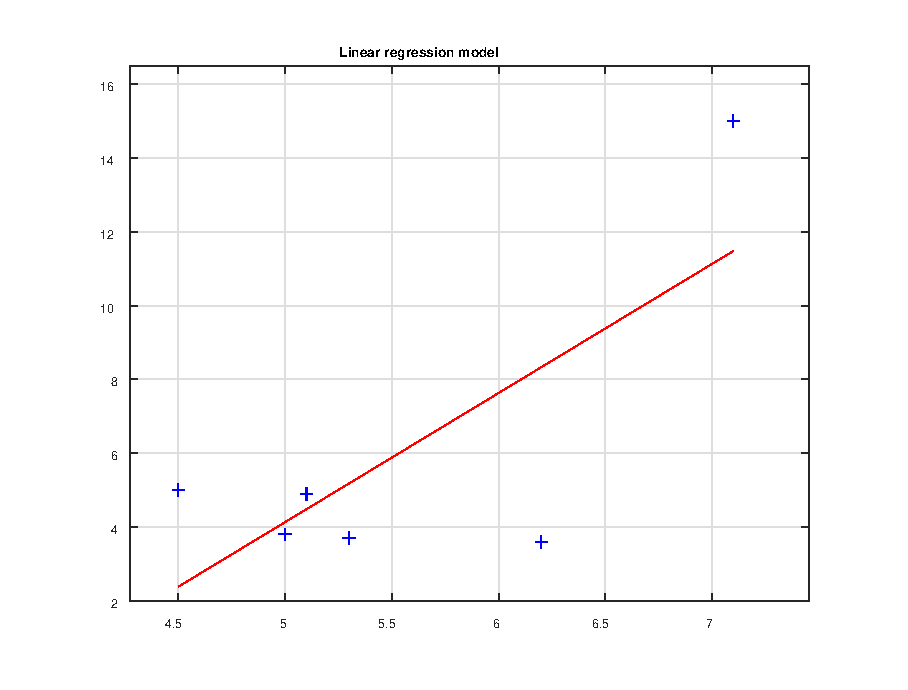
\includegraphics[width=\maxwidth{56.196688409433015em}]{figure_0.eps}
\end{center}

\label{H_927089EF}
\matlabheadingthree{a) The sum of the squared error}

\begin{par}
\begin{flushleft}
Firstly, we define an anonymous function with the unconstrained optimization problem we are trying to solve. We set the parameters that are not objects of the problem by overriding them in a new function. Finally, we solve the optimization problem by defining a pair of initial values as a starting point.
\end{flushleft}
\end{par}

\begin{matlabcode}
f = @(x,y,beta) sum((y - beta(1) - beta(2).*x).^2)
\end{matlabcode}
\begin{matlaboutput}
f = 
    @(x,y,beta)sum((y-beta(1)-beta(2).*x).^2)

\end{matlaboutput}
\begin{matlabcode}
myfunc = @(beta) f(x,y,beta)
\end{matlabcode}
\begin{matlaboutput}
myfunc = 
    @(beta)f(x,y,beta)

\end{matlaboutput}

\begin{par}
\begin{flushleft}
It can be resolved with two different methods natively in MATLAB: \texttt{fminunc} and \texttt{fminsearch}. We will get the same result.
\end{flushleft}
\end{par}

\begin{matlabcode}
fminunc(myfunc,[0,0]) % using a gradient boot search method
\end{matlabcode}
\begin{matlaboutput}
Local minimum found.

Optimization completed because the size of the gradient is less than
the value of the optimality tolerance.

<stopping criteria details>
ans = 1x2    
  -13.3585    3.4985

\end{matlaboutput}
\begin{matlabcode}
bopt1 = fminsearch(myfunc,[0,0]) % using derivative-free method
\end{matlabcode}
\begin{matlaboutput}
bopt1 = 1x2    
  -13.3585    3.4985

\end{matlaboutput}

\begin{par}
\begin{flushleft}
We have obtained the following values:
\end{flushleft}
\end{par}

\begin{par}
$$\begin{array}{l}
\alpha =-13\ldotp 3585\\
\beta =3\ldotp 4985
\end{array}$$
\end{par}

\label{H_ADE52C10}
\matlabheadingthree{b) The sum of the absolute value of the errors.}

\begin{par}
\hfill \break
\end{par}

\begin{matlabcode}
f2 = @(x,y,beta) sum(abs((y - beta(1) - beta(2).*x)))
\end{matlabcode}
\begin{matlaboutput}
f2 = 
    @(x,y,beta)sum(abs((y-beta(1)-beta(2).*x)))

\end{matlaboutput}
\begin{matlabcode}
myfunc2 = @(beta) f2(x,y,beta)
\end{matlabcode}
\begin{matlaboutput}
myfunc2 = 
    @(beta)f2(x,y,beta)

\end{matlaboutput}
\begin{matlabcode}
bopt2 = fminsearch(myfunc2,[0,0])
\end{matlabcode}
\begin{matlaboutput}
bopt2 = 1x2    
  -22.8665    5.3333

\end{matlaboutput}

\begin{par}
\begin{flushleft}
With this method, we have obtained:
\end{flushleft}
\end{par}

\begin{par}
$$\begin{array}{l}
\alpha =-22\ldotp 8665\\
\beta =5\ldotp 3333
\end{array}$$
\end{par}

\begin{par}
\begin{flushleft}
\underline{\textbf{Using the linear programming method}}
\end{flushleft}
\end{par}

\begin{par}
\begin{flushleft}
\hyperref[H_62E93EF6]{\textit{See in the appendix the general structure of a LP problem.}}
\end{flushleft}
\end{par}

\begin{par}
\begin{flushleft}
The optimization problem can be defined as
\end{flushleft}
\end{par}

\begin{par}
$$\min_{\alpha ,\beta } \sum_i^n |\epsilon_i |$$
\end{par}

\begin{par}
\begin{flushleft}
Being
\end{flushleft}
\end{par}

\begin{par}
$$\epsilon_i =y_i -{\hat{y} }_i =y_i -\alpha -\beta x_i$$
\end{par}

\begin{par}
\begin{flushleft}
Since we want to formulate it as a linear programming problem, we have to make a change of variable to leave it in linear terms. This implies that we have to define two new constraints:
\end{flushleft}
\end{par}

\begin{par}
$$u_i \le \;|\epsilon_i |=\left\lbrace \begin{array}{ll}
u_i =\left(y_i -{\hat{y} }_i \right)=y_i -\alpha -\beta x_i \le \epsilon_i  & i=1,\ldots,n\\
u_i ={-\epsilon }_i =-\left(y_i -{\hat{y} }_i \right)=-\left(y_i -\alpha -\beta x_i \right)\ge -\epsilon_i  & i=1,\ldots,n
\end{array}\right.$$
\end{par}

\begin{par}
\begin{flushleft}
With the condition that the absolute value is always positive, our LP problem is:
\end{flushleft}
\end{par}

\begin{par}
$$\begin{array}{l}
\min_{u_1 ,\ldots,u_n ,\alpha ,\beta } \sum_i^n u_i \\
{\textrm{s.}\;\textrm{to}}\\
i)-u_i -\alpha -\beta x_i \le -y_i ,~~\forall i=1,...,n\\
ii)-u_i +\alpha +\beta x_i \le y_i ,~~\forall i=1,...,n\\
iii)\;u_i \ge 0
\end{array}$$
\end{par}

\begin{par}
\begin{flushleft}
In our concrete case, $n=6$. 
\end{flushleft}
\end{par}

\begin{par}
\begin{flushleft}
Therefore, we have 8 decision variables ($u_1 ,u_2 ,u_3 ,u_4 ,u_5 ,u_6 ,\alpha ,\beta$), 12 inequations, and an inferior bound for each $u_i$. 
\end{flushleft}
\end{par}

\begin{matlabcode}
n = length(x)
\end{matlabcode}
\begin{matlaboutput}
n = 6
\end{matlaboutput}
\begin{matlabcode}
u = (-1)*diag(ones(n,1));
Aub = zeros(12,8);
for i = 1:n
    Aub(i,:) = [u(i,:),-1,-x(i)];
    Aub(6+i,:) = [u(i,:),1,x(i)];
end
Aub
\end{matlabcode}
\begin{matlaboutput}
Aub = 12x8    
   -1.0000         0         0         0         0         0   -1.0000   -4.5000
         0   -1.0000         0         0         0         0   -1.0000   -5.0000
         0         0   -1.0000         0         0         0   -1.0000   -5.1000
         0         0         0   -1.0000         0         0   -1.0000   -5.3000
         0         0         0         0   -1.0000         0   -1.0000   -6.2000
         0         0         0         0         0   -1.0000   -1.0000   -7.1000
   -1.0000         0         0         0         0         0    1.0000    4.5000
         0   -1.0000         0         0         0         0    1.0000    5.0000
         0         0   -1.0000         0         0         0    1.0000    5.1000
         0         0         0   -1.0000         0         0    1.0000    5.3000

\end{matlaboutput}
\begin{matlabcode}
b = [-y;y]
\end{matlabcode}
\begin{matlaboutput}
b = 12x1    
   -5.0000
   -3.8000
   -4.9000
   -3.7000
   -3.6000
  -15.0000
    5.0000
    3.8000
    4.9000
    3.7000

\end{matlaboutput}
\begin{matlabcode}
c = [ones(1,n),[0,0]]
\end{matlabcode}
\begin{matlaboutput}
c = 1x8    
     1     1     1     1     1     1     0     0

\end{matlaboutput}
\begin{matlabcode}
lin_pr = linprog(c,Aub,b);
\end{matlabcode}
\begin{matlaboutput}
Optimal solution found.
\end{matlaboutput}
\begin{matlabcode}
bopt2lin = lin_pr(end-1:end)
\end{matlabcode}
\begin{matlaboutput}
bopt2lin = 2x1    
  -22.8667
    5.3333

\end{matlaboutput}

\begin{par}
\begin{flushleft}
Solving as an LP problem, we have obtained the following values:
\end{flushleft}
\end{par}

\begin{par}
$$\begin{array}{l}
\alpha =-22\ldotp 8667\\
\beta =5\ldotp 3333
\end{array}$$
\end{par}

\label{H_609B43E2}
\matlabheadingthree{c) The maximum of the absolute values of the errors.}

\begin{par}
\hfill \break
\end{par}

\begin{matlabcode}
f3 = @(x,y,beta) max(abs((y - beta(1) - beta(2).*x)))
\end{matlabcode}
\begin{matlaboutput}
f3 = 
    @(x,y,beta)max(abs((y-beta(1)-beta(2).*x)))

\end{matlaboutput}
\begin{matlabcode}
myfunc3 = @(beta) f3(x,y,beta)
\end{matlabcode}
\begin{matlaboutput}
myfunc3 = 
    @(beta)f3(x,y,beta)

\end{matlaboutput}
\begin{matlabcode}
bopt3 = fminsearch(myfunc3,[0,0])
\end{matlabcode}
\begin{matlaboutput}
bopt3 = 1x2    
  -16.2769    3.8462

\end{matlaboutput}

\begin{par}
\begin{flushleft}
Obtaining:
\end{flushleft}
\end{par}

\begin{par}
$$\begin{array}{l}
\alpha =-16\ldotp 2769\\
\beta =3\ldotp 8462
\end{array}$$
\end{par}

\label{H_FBADF982}
\matlabheadingthree{Plotting the solutions}

\begin{par}
\hfill \break
\end{par}

\begin{matlabcode}
reg1 = bopt1(1) + bopt1(2)*x;
reg2 = bopt2(1) + bopt2(2)*x;
reg3 = bopt3(1) + bopt3(2)*x;
\end{matlabcode}

\begin{par}
$$\left\lbrace \begin{array}{c}
y_1 =-13.36+3.50x\\
y_2 =-22.87+5.33x\\
y_3 =-16.28+3.85x
\end{array}\right.$$
\end{par}

\begin{matlabcode}
plot(x,y,'b*',x,reg1,'-r',x,reg2,'--g',x,reg3,'-.k')
legend('original points','a)','b)','c)')
xlim([min(x),max(x)])
ylim([2,max(y)*1.1])
title('Comparison between the three types of regression line models')
\end{matlabcode}
\begin{center}
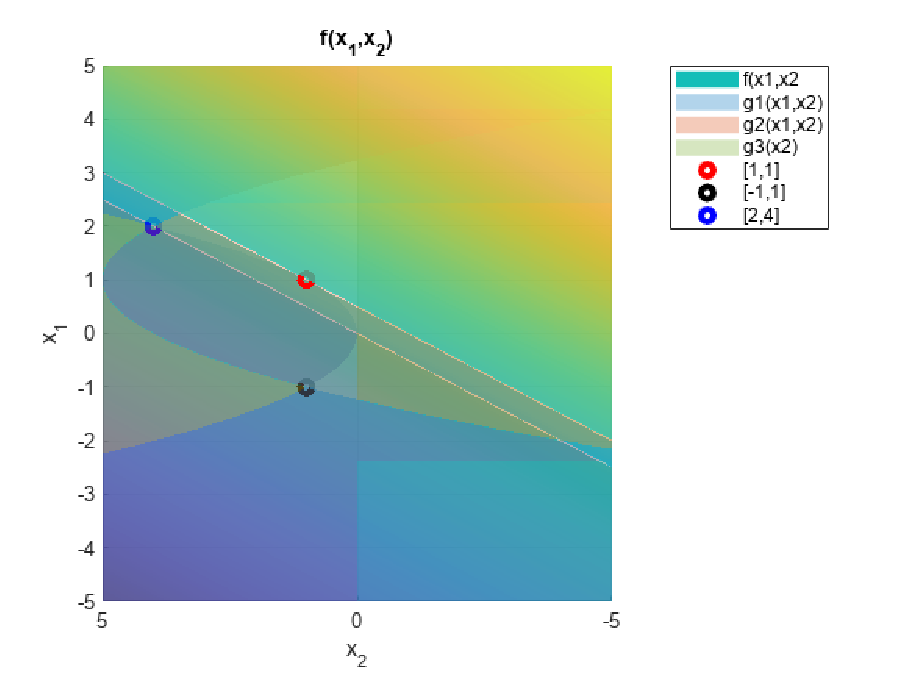
\includegraphics[width=\maxwidth{56.196688409433015em}]{figure_1.eps}
\end{center}

\begin{par}
\begin{flushleft}
We can observe that the regression lines are strongly influenced by a point that could be considered an outlier. Depending on the optimization method, the influence of this point is lower or higher. The other points are much nearer; if we had analyzed only those points, the regression line would have been a less pronounced slope.
\end{flushleft}
\end{par}


\label{H_8D056BE4}
\matlabheading{Appendix}

\label{H_62E93EF6}
\matlabheadingtwo{Linear Programming Problem structure}

\begin{par}
\begin{flushleft}
\includegraphics[width=\maxwidth{20.471650777722026em}]{image_0}
\end{flushleft}
\end{par}

\end{document}
